We now constrain some generic DM candidates which will ignite a WD via one of the processes parameterized in Section~\ref{sec:dmignition}.
These release SM particles that deposit their energy and thermalize ions within a distance described in Section~\ref{sec:smheating}.
First, however, we review how WD observables constrain DM candidates capable of triggering SN.

\subsection{Review of WD Observables}
Following the discussion of~\cite{Graham:2015apa}, our constraints come from (1)~the existence of heavy, long-lived white dwarfs, or (2)~the measured type Ia SN rate.
The typical age of a WD is of order the age of the universe $\sim \text{Gyr}$.
RX~J0648.04418 is a nearby star and one of the heavier known WDs, with a mass $\sim 1.25 ~M_{\astrosun}$~\cite{Mereghetti:2013nba} and local dark matter density which we take to be $\rho_\chi \sim 0.4 ~\GeV/\text{cm}^3$.
Of course, this is not the only known heavy WD---the Sloan Digital Sky Survey~\cite{SDSS} has found $20+$ others.
% https://heasarc.gsfc.nasa.gov/db-perl/W3Browse/w3hdprods.pl
The NuStar collaboration has also recently uncovered evidence for the likely existence of heavy WDs near the galactic center~\cite{NuStar}, where the DM density is assumed to be much greater $\rho_\chi \gtrsim 10^3 ~\text{GeV}/\text{cm}^3$~\cite{Nesti:2013uwa}.
Such heavy candidates are particularly suited for our constraints as the energy deposit necessary to trigger SN~\eqref{eq:energy_boom_condition} is a decreasing function of WD mass.
However, less dense white dwarfs are significantly more abundant in the galaxy.
Thus, even if a sufficiently massive DM is unable to trigger a violent heating event within the lifetime of a WD, it could still ignite enough lighter WDs to affect the measured SN rate of $\sim $ 0.3 per century.
The DM-induced SN rate is estimated using the expected number of white dwarfs per galaxy $\sim 10^{10}$ and their mass distribution~\cite{SDSS}.
Simulations indicate that only WD masses heavier than $\sim 0.85 ~M_{\astrosun}$ will result in optically visible SN~\cite{Graham:2015apa}.
Therefore, most of the stars exploded in this manner will be in the mass range $\sim 0.85 - 1 ~M_{\astrosun}$, resulting in weaker SN than expected of typical Chandrasekhar mass WDs.

To summarize, a bound on DM parameters can be placed if either a single explosive event occurs during the lifetime of an observed star such as RX~J0648.04418, or the SN rate due to such DM events throughout the galaxy exceeds the measured value.
Note that for low-mass WDs dominated by photon diffusion, $\Eboom$ is a strong function of WD density.
The average density for WDs is typically a factor $\sim 10^{-2} - 10^{-1}$ less than the central density, although it is found that the WD density only changes by an $\OO(1)$ fraction from the central value up to a distance $\sim R_\text{WD}/2$~\cite{Chandrasekhar}.
Therefore the central density is a valid approximation as long as we consider heating events within this ``modified" WD volume.
For simplicity, we employ this approach.

\subsection{Scattering Constraints}
\label{sec:TransitConstraints}

In order to constrain a DM model with a scattering interaction, we require that it satisfy the ignition condition~\eqref{eq:transitexplosion}.
This is given in terms of an LET, which parameterizes the ability for DM to release sufficient energy to the star in the form of SM particles.
Here we consider a DM elastic scattering off carbon ions with cross section $\sigma_{\chi A}$, which has an LET:
\begin{align}
\label{eq:schematicLET}
  \left( \frac{d E}{d x} \right)_\text{LET} \sim n_\text{ion} \sigma_{\chi A} m_\text{ion} v_\text{esc}^2.
\end{align}
This can be expressed in terms of the cross section per nucleon $\sigma_{\chi n}$---see Appendix \ref{sec:capture}
Each elastic scatter transfers an energy of order $m_\text{ion} v_\text{esc}^2 \approx 1-10~\text{MeV}$ to the target nuclei, thus enabling fusion reactions.
Note that the stopping power of the DM in the non-degenerate envelope is of the same form, but with the density replaced by its diminished value in this region.
It is interesting that combining the ignition condition~\eqref{eq:transitexplosion} with the requirement that the DM adequately penetrates the non-degenerate layer~\eqref{eq:CrustCondition} yields a lower bound on DM mass.
\begin{align}
\label{eq:transitmass}
m_\chi > \Eboom \l \frac{R_\text{env}}{\lambda_T} \r \l \frac{\rho_\text{env}}{\rho_\text{WD}} \r \frac{1}{v_\text{esc}^2},
\end{align}
where $\rho_\text{WD}$ is the central density of the WD.
Here $R_\text{env} \approx 50 ~\text{km}$ is the width of a non-degenerate WD envelope---the density in this region $\rho_\text{env}$ is typically a small fraction $\sim 10^{-3}$ of the central density~\cite{KippenhahnWeigert}.
We conservatively take the envelope to be composed of carbon ions; if it were primarily hydrogen or helium, then the condition for penetration is weakened by 4 orders of magnitude due to the reduced energy transfer and cross section for scattering.
We find that the DM must be heavier than $\sim 10^{28} ~\GeV$ to ensure an explosive transit of a $1.25~M_{\astrosun}$ WD \emph{and} minimal loss of kinetic energy in the non-degenerate layer.

Of course, this bound is only applicable if the energy input to the WD is solely coming from DM kinetic energy.
We may also consider DM inelastic scattering off carbon ions which transfer more than $\sim \text{MeV}$ per collision.
Examples of such a process include baryon-number violating interactions which can release the nucleon mass energy $\sim \GeV$ per collision.
This is similar to Q-balls, which absorb the baryon number of nuclear targets and liberate binding energy rather than transferring kinetic energy---this interaction is examined in Section~\ref{sec:qballs}.
Note that the assumption of a ``point-like" interaction requires that the physical size of the DM is much smaller than $\lambda_T$---this is sensible up to masses of order $\sim 10^{47}~\GeV$, at which point the gravitational radius of the DM exceeds $\lambda_T$.

In Figure~\ref{fig:transit-elastic} we constrain the DM elastic scattering cross section per nucleon $\sigma_{\chi n}$ as a function of DM mass $m_\chi$ using the different classes of observables described above.
Note that the scattering cross sections constrained here are incredibly large $\gtrsim 10^{-10} ~\cm^2$---however, the constraints from WDs reach to very large masses for which no other constraints exist.
At these masses, the most stringent limits on DM elastic scattering are from CMB and Lyman-$\alpha$ spectrum analysis~\cite{Dvorkin:2013cea}, which constrain $\frac{\sigma_{\chi n}}{m_\chi} < \frac{10^{-3} \text{b}}{\GeV}$. 
These cross-sections also require that the DM involved be macroscopically large, of order or larger than the trigger size, and so the interaction is decidedly not ``point-like.''
This fact does not weaken our constraints, however, since the energy transferred to each ion in the DM's path is greater than $\sim \text{MeV}$.

\begin{figure}
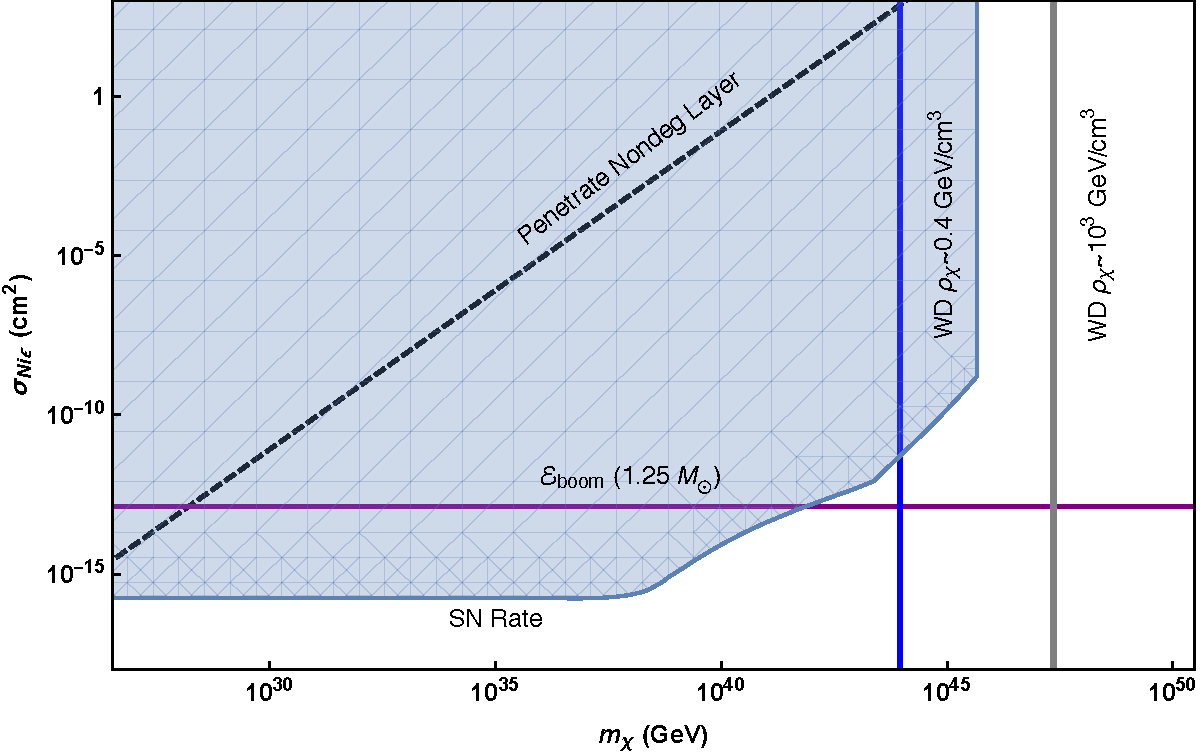
\includegraphics[scale=.45]{transitobservation.pdf}
\caption{Constraints on DM-carbon elastic scattering cross-section.
Bounds come from demanding that the DM transit triggers runaway fusion~\eqref{eq:transitexplosion} and occurs at a rate~\eqref{eq:TransitRate} large enough to either ignite a $1.25~M_{\astrosun}$ WD in its lifetime or exceed the measured SN rate in our galaxy (blue shaded).
We also demand that the DM penetrates the non-degenerate stellar envelope, taken at the highest densities, without losing appreciable kinetic energy.
Constraints from the CMB/large-scale structure~\cite{Dvorkin:2013cea} are depicted as well.
}
\label{fig:transit-elastic}
\end{figure}

\subsection{Collision and Decay Constraints}
\label{sec:CollisionConstraints}

In order to constrain a DM model through its annihilations or decays within a WD, we require that it satisfy the ignition condition~\eqref{eq:coldecay}.
Consider a single annihilation or decay with $f_\text{SM} = 1$ that releases a spectrum of SM particles.
As shown in Section~\ref{sec:smheating}, the constraint has minimal dependence on the released species if the typical energy $\epsilon$ of secondary products is greater than an MeV.
In the case of neutrinos, we may simply demand that $\epsilon$ is sufficiently large that a single neutrino can ignite the star.
With this schematic for the DM interaction, we can constrain the cross section for collision $\sigma_{\chi \chi}$ and lifetime $\tau_\chi$.
This is done in Figures~\ref{fig:transit-collision} and~\ref{fig:transit-decay} in the case of transiting DM using the different classes of observables for DM-DM collisions and DM decays, respectively.

Of course there are existing limits on DM annihilations and decays, complementary to the ones placed from WDs.
DM annihilations/decays inject energy and affect the ionization history of our universe, which can be probed by measurements of the CMB temperature and polarization angular spectrum \cite{Padmanabhan:2005es, Slatyer:2009yq, Slatyer:2016qyl}.
These constraints are of order $\sigma_{\chi \chi} v < 10^{-27} ~\frac{\cm^3}{\text{s}} \l \frac{m_\chi}{10 ~\GeV} \r$ for annihilations, and  $\tau_\chi > 10^{7} ~\text{Gyr}$ for decay.
There are also constraints on DM annihilation/decays in our halo from the cosmic ray (CR) flux seen in large terrestrial detectors.
Here we provide a crude estimate of the expected constraints from CRs in the case of DM annihilation (decays are qualitatively similar).
A more detailed analysis is beyond the scope of this work.
The Pierre Auger Observatory \cite{ThePierreAuger:2015rma} has detected the flux of $E_\text{th} \sim 10^{11} ~\GeV$ cosmic rays with an exposure of order $A_\text{PA} \sim 40000 ~\text{km}^2 ~\text{sr} ~\text{yr}$.
Ultra-heavy DM annihilations $m_\chi > 10^{16} ~\GeV$ will generally produce secondary particles of energy $\epsilon \gtrsim E_\text{th}$ via final-state radiation.
For a simple 2-2 process (e.g. $\chi \chi \to q q$), the expected number of final-state particles radiated at $E_\text{th}$ due to QCD showers is approximated by the Sudakov double logarithm
\begin{equation}
N_\text{rad} \sim \frac{4 \alpha_s}{\pi} \log\l\frac{m_\chi}{\Lambda_\text{QCD}}\r \log\l\frac{m_\chi}{E_\text{th}}\r \approx 100,
\end{equation}
where $\alpha_s$ is the QCD coupling constant.
Similarly, the estimated number of final-state particles at $E_\text{th}$ due to EW showers is $\approx 50$.
We expect that CRs at this energy originating in our galaxy will be able to strike the earth unattenuated.
Thus, such events would affect the measured CR flux of Pierre Auger unless
\begin{equation}
\l \frac{\rho_\chi}{m_\chi}\r^2 \sigma_{\chi \chi} v \frac{R_\text{halo}}{4 \pi} N_\text{rad} \times A_\text{PA} \lesssim 1.
\end{equation}
Here we assume an average value for DM density $\rho_\chi \approx 0.4~\GeV/\cm^3$ as a reasonable approximation to the integral over our galactic halo volume.
Surprisingly, the above CR constraints are (within a few orders of magnitude) comparable to the constraints due to the observation of long-lived WDs.
This is actually due to a coincidence in the effective ``space-time volumes" of the two systems.
A terrestrial CR detector such as Pierre Auger sees events within a space-time volume $(R_\text{det}^2 R_\text{halo} \times t_\text{det})$, where $R_\text{det} \sim 50 ~\text{km}$, $R_\text{halo} \sim 10 ~\text{kpc}$, and $t_\text{det} \sim 10 ~\text{yr}$.
This is similar in magnitude to the WD space-time volume $(R_\text{WD}^3 \times \tau_\text{WD})$.

In the case of captured DM, we show the constraints on $\sigma_{\chi \chi}$ and $\tau_\chi$ assuming a benchmark value of the elastic scattering cross section $\sigma_{\chi n} = 10^{-32} ~\cm^2$.
With regards to DM-DM collisions, we also assume a stabilizing radius for the collapsing DM sphere. 
This is done in Figures~\ref{fig:capture-collision} and~\ref{fig:capture-decay}---for simplicity, here we only show the constraints from the existence of nearby, heavy WDs.

It is important to note that there is a large parameter space in $\sigma_{\chi n}$ which will lead to DM capture, thermalization, and core collapse in a WD.
This is depicted in Figure~\ref{fig:elastic-capture}, along with the existing constraints on DM elastic scattering.
As detailed in~\cite{Mack:2007xj}, direct detection experiments such as Xenon 1T~\cite{Aprile:2017iyp} are only sensitive to DM masses $m_\chi < 10^{17} ~\GeV$.
For even larger masses $m_\chi < 10^{26} ~\GeV$ there are constraints from the MACRO experiment \cite{Ambrosio:2002qq} and from ancient excavated mica.
The latter has been studied in~\cite{Jacobs:2014yca}.
We have similarly estimated the bounds from MACRO assuming a detectable threshold of $\sim 5~\text{MeV}/\cm$~\cite{Ambrosio:2002qq}.

\begin{figure}
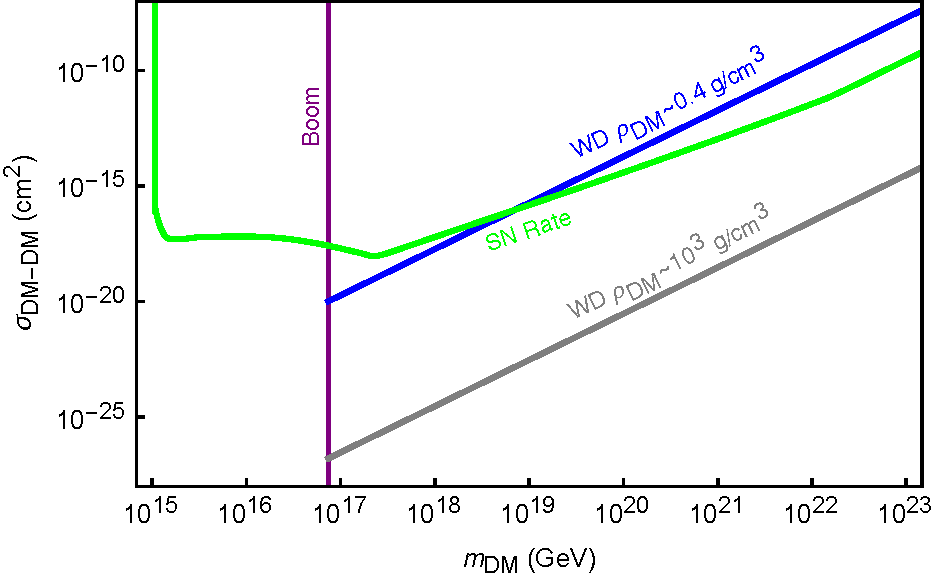
\includegraphics[scale=.45]{collisionobservation.pdf}
\caption{Constraints on DM-DM collision cross-section to SM products of energy $\epsilon \gg \MeV$.
Bounds come from demanding that the DM transit interaction triggers runaway fusion~\eqref{eq:coldecay} and occurs at a rate~\eqref{eq:collisionDM} large enough to either ignite an observed $1.25~M_{\astrosun}$ WD in its lifetime or exceed the measured SN rate in our galaxy (blue shaded).
Also shown are the CMB \cite{Slatyer:2009yq} (red) and CR flux (black) constraints on DM annihilations.}
\label{fig:transit-collision}
\end{figure}

\begin{figure}
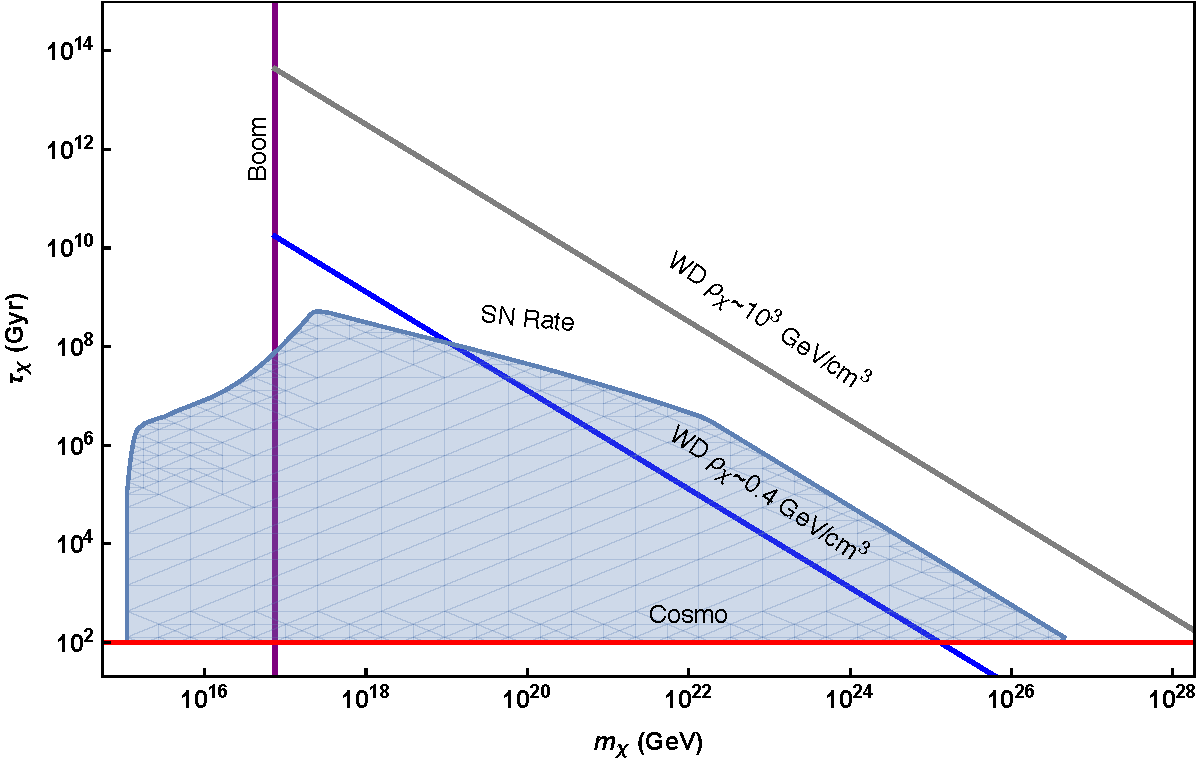
\includegraphics[scale=.45]{decayobservation.pdf}
\caption{Constraints on DM decay to SM products of energy $\epsilon \gg \MeV$.
Bounds come from demanding that the DM transit interaction triggers runaway fusion~\eqref{eq:coldecay} and occurs at a rate~\eqref{eq:decayDM} large enough to either ignite an observed $1.25~M_{\astrosun}$ WD in its lifetime or exceed the measured SN rate in our galaxy (blue shaded).
Also shown are the CMB \cite{Slatyer:2016qyl} (red) and CR flux (black) constraints on DM lifetime.}
\label{fig:transit-decay}
\end{figure}

\begin{figure}
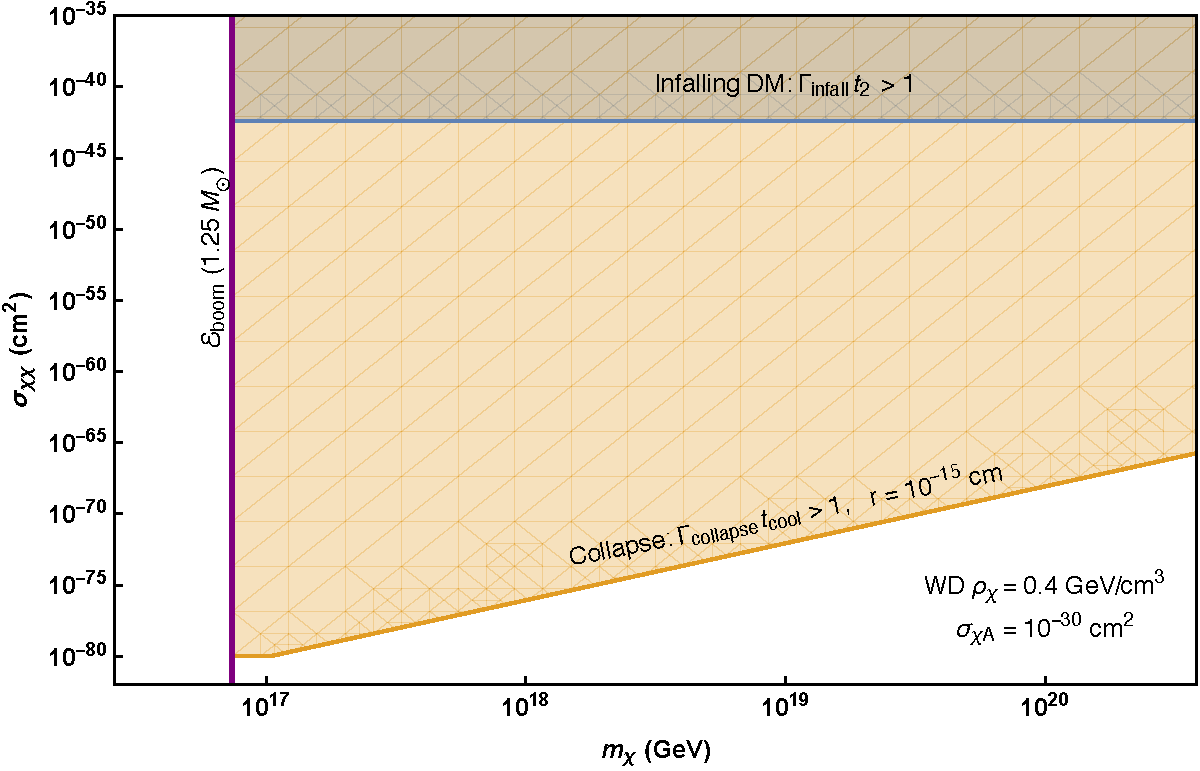
\includegraphics[scale=.45]{capturecollision.pdf}
\caption{Constraints on DM-DM collision cross-section to SM products of energy $\epsilon \gg \MeV$, assuming DM is captured with an elastic scattering $\sigma_{\chi n} = 10^{-32} ~\cm^2$.
Bounds come from the observation of $1.25~M_{\astrosun}$ WDs in local DM density.
We consider the annihilation rate during the in-falling thermalization stage~\eqref{eq:infall} (blue shaded) and during self-gravitational collapse~\eqref{eq:collapse} to a stable radius $r = 10^{-10} ~\cm$ (green shaded). See text for details.
}
\label{fig:capture-collision}
\end{figure}

\begin{figure}
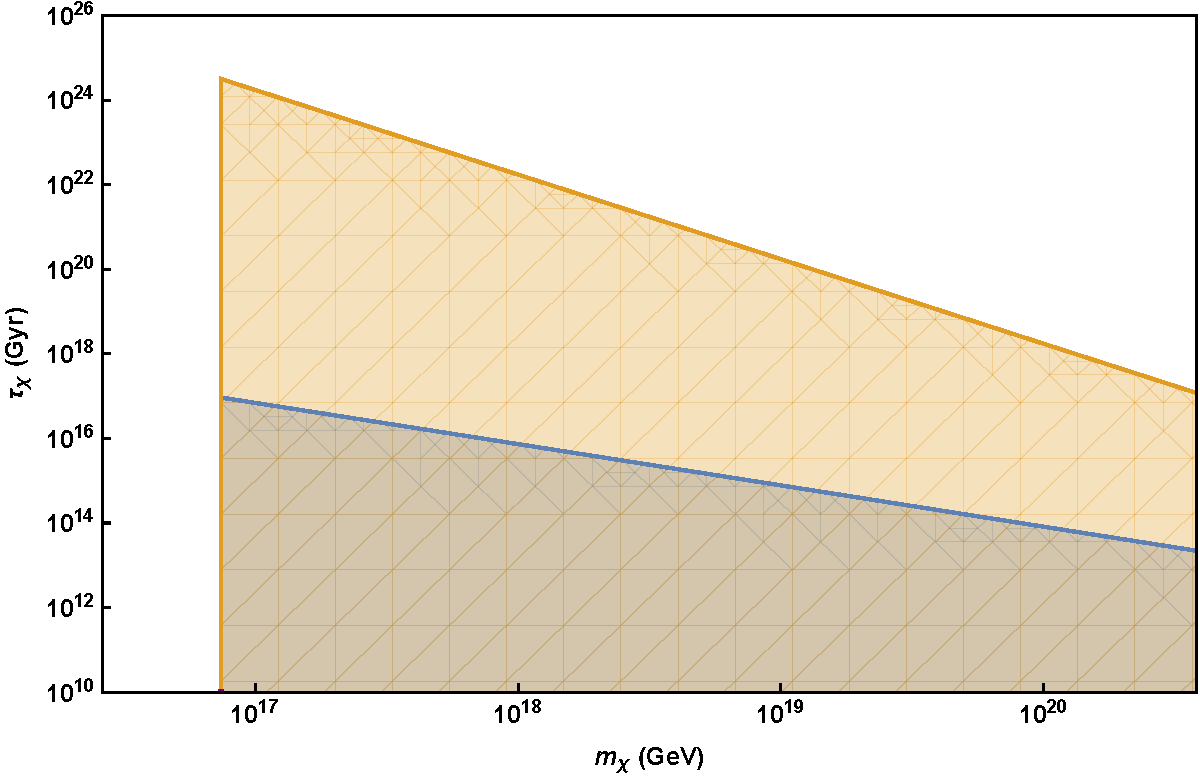
\includegraphics[scale=.45]{capturedecay.pdf}
\caption{Constraints on DM decay to SM products of energy $\epsilon \gg \MeV$, assuming DM is captured with an elastic scattering $\sigma_{\chi n} = 10^{-32} ~\cm^2$.
Bounds come from the observation of $1.25~M_{\astrosun}$ WDs in local DM density.
We consider the rate of decays during the in-falling thermalization stage (blue shaded) and for a decaying DM core (green shaded). See text for details.
}
\label{fig:capture-decay}
\end{figure}

\begin{figure}
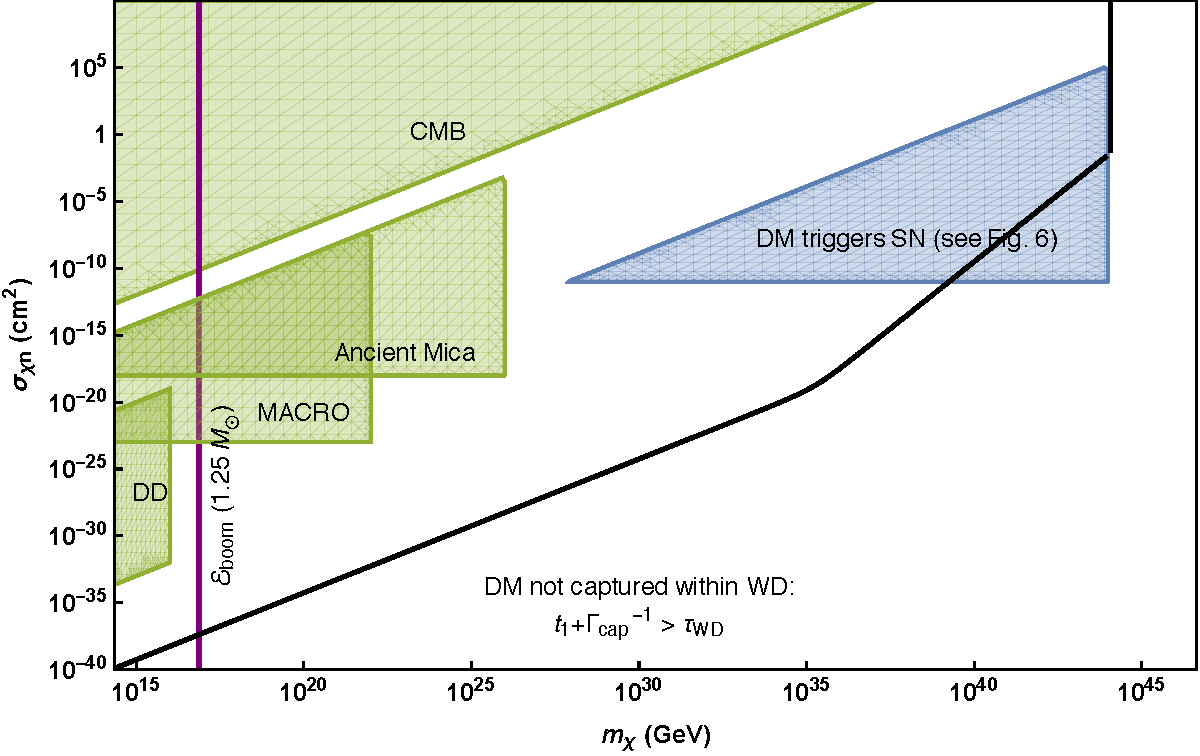
\includegraphics[scale=.45]{elasticcapture.pdf}
\caption{Viable parameter space (above the black line) in which DM-nucleon elastic scattering leads to DM capture in a $1.25 ~M_{\astrosun}$ WD.  All of this space is subject to constraints on DM decay and DM-DM annihilation analogous to those given in Figures~\ref{fig:capture-decay} and~\ref{fig:capture-collision}.  Note the blue region, reproducing Figure~\ref{fig:transit-elastic}, indicates DM which causes SN via elastic heating. 
We also indicate here an estimate of the scattering constraints from cosmology, direct detection, MACRO, and ancient mica \cite{Jacobs:2014yca}.}
\label{fig:elastic-capture}
\end{figure}
